\documentclass{standalone}
\usepackage{tikz}
\begin{document}
    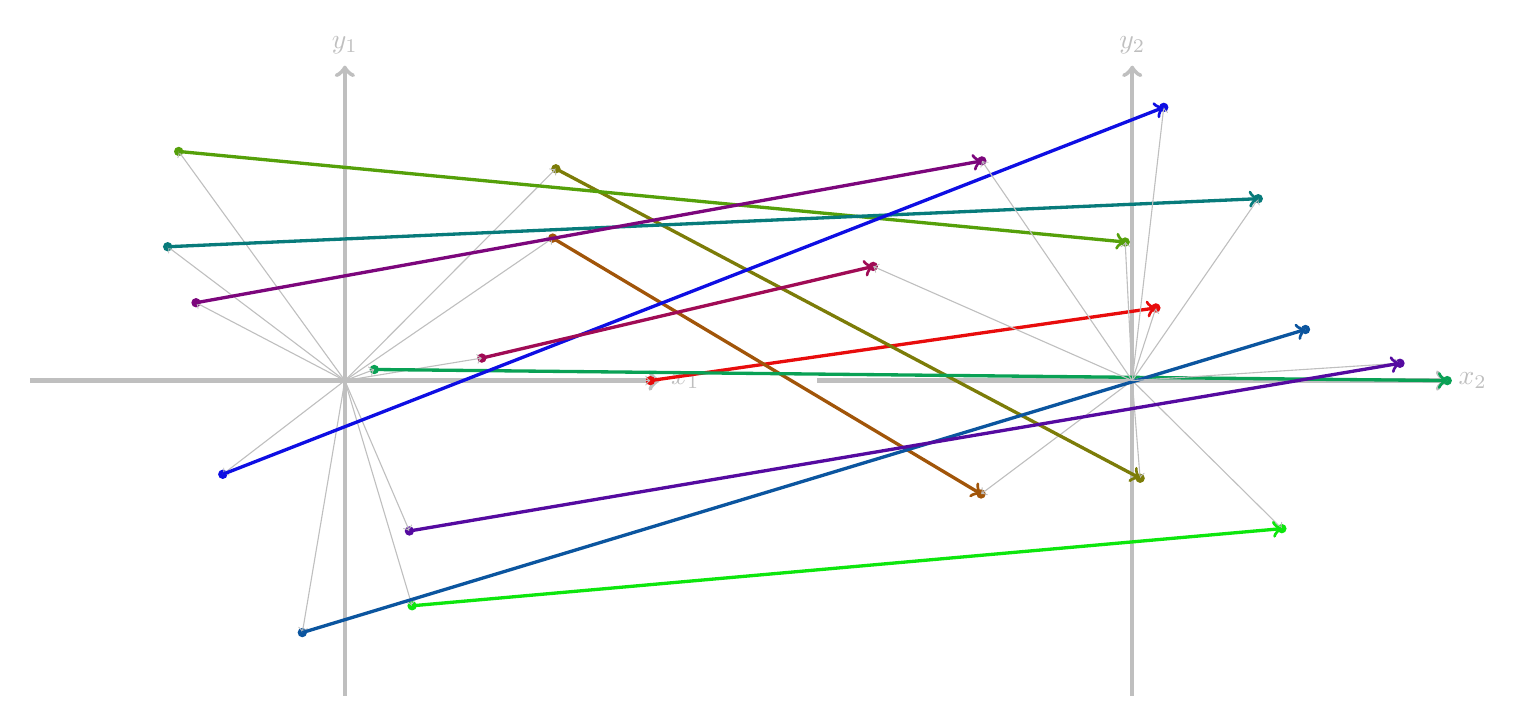
\begin{tikzpicture}

        \draw[->,ultra thick, lightgray] (-4.0,0)--(4.0,0) node[right]{$x_1$};
        \draw[->,ultra thick, lightgray] (0.0,-4)--(0.0,4) node[above]{$y_1$};

        \node at (3.88,-2.56e-17)[circle,fill={rgb:red,0.318;green,0.0161;blue,0.0161},inner sep=1.2pt]{};

        \draw[->, thin, color=lightgray] (0.0,0.0) -- (3.88, -2.56e-17);

        \node at (2.64,1.81)[circle,fill={rgb:red,0.318;green,0.168;blue,0.0185},inner sep=1.2pt]{};

        \draw[->, thin, color=lightgray] (0.0,0.0) -- (2.64, 1.81);

        \node at (2.68,2.69)[circle,fill={rgb:red,0.318;green,0.318;blue,0.0204},inner sep=1.2pt]{};

        \draw[->, thin, color=lightgray] (0.0,0.0) -- (2.68, 2.69);

        \node at (-2.11,2.91)[circle,fill={rgb:red,0.169;green,0.317;blue,0.0203},inner sep=1.2pt]{};

        \draw[->, thin, color=lightgray] (0.0,0.0) -- (-2.11, 2.91);

        \node at (0.854,-2.86)[circle,fill={rgb:red,0.0175;green,0.317;blue,0.0175},inner sep=1.2pt]{};

        \draw[->, thin, color=lightgray] (0.0,0.0) -- (0.854, -2.86);

        \node at (0.374,0.141)[circle,fill={rgb:red,0.0186;green,0.317;blue,0.168},inner sep=1.2pt]{};

        \draw[->, thin, color=lightgray] (0.0,0.0) -- (0.374, 0.141);

        \node at (-2.25,1.7)[circle,fill={rgb:red,0.0216;green,0.317;blue,0.317},inner sep=1.2pt]{};

        \draw[->, thin, color=lightgray] (0.0,0.0) -- (-2.25, 1.7);

        \node at (-0.54,-3.2)[circle,fill={rgb:red,0.0213;green,0.17;blue,0.318},inner sep=1.2pt]{};

        \draw[->, thin, color=lightgray] (0.0,0.0) -- (-0.54, -3.2);

        \node at (-1.55,-1.19)[circle,fill={rgb:red,0.0197;green,0.0197;blue,0.318},inner sep=1.2pt]{};

        \draw[->, thin, color=lightgray] (0.0,0.0) -- (-1.55, -1.19);

        \node at (0.82,-1.91)[circle,fill={rgb:red,0.169;green,0.0207;blue,0.317},inner sep=1.2pt]{};

        \draw[->, thin, color=lightgray] (0.0,0.0) -- (0.82, -1.91);

        \node at (-1.89,0.989)[circle,fill={rgb:red,0.318;green,0.016;blue,0.318},inner sep=1.2pt]{};

        \draw[->, thin, color=lightgray] (0.0,0.0) -- (-1.89, 0.989);

        \node at (1.74,0.286)[circle,fill={rgb:red,0.318;green,0.021;blue,0.169},inner sep=1.2pt]{};

        \draw[->, thin, color=lightgray] (0.0,0.0) -- (1.74, 0.286);

        \draw[->,ultra thick, lightgray] (6.0,0)--(14.0,0) node[right]{$x_2$};
        \draw[->,ultra thick, lightgray] (10.0,-4)--(10.0,4) node[above]{$y_2$};

        \node at (10.3,0.923)[circle,fill={rgb:red,0.318;green,0.0161;blue,0.0161},inner sep=1.2pt]{};

        \draw[->, thin, color=lightgray] (10.0,0.0) -- (10.3, 0.923);

        \draw[->, very thick, color={rgb:red,0.318;green,0.0161;blue,0.0161}] (3.88,-2.56e-17) -- (10.3, 0.923);

        \node at (8.08,-1.44)[circle,fill={rgb:red,0.318;green,0.168;blue,0.0185},inner sep=1.2pt]{};

        \draw[->, thin, color=lightgray] (10.0,0.0) -- (8.08, -1.44);

        \draw[->, very thick, color={rgb:red,0.318;green,0.168;blue,0.0185}] (2.64,1.81) -- (8.08, -1.44);

        \node at (10.1,-1.24)[circle,fill={rgb:red,0.318;green,0.318;blue,0.0204},inner sep=1.2pt]{};

        \draw[->, thin, color=lightgray] (10.0,0.0) -- (10.1, -1.24);

        \draw[->, very thick, color={rgb:red,0.318;green,0.318;blue,0.0204}] (2.68,2.69) -- (10.1, -1.24);

        \node at (9.91,1.76)[circle,fill={rgb:red,0.169;green,0.317;blue,0.0203},inner sep=1.2pt]{};

        \draw[->, thin, color=lightgray] (10.0,0.0) -- (9.91, 1.76);

        \draw[->, very thick, color={rgb:red,0.169;green,0.317;blue,0.0203}] (-2.11,2.91) -- (9.91, 1.76);

        \node at (11.9,-1.88)[circle,fill={rgb:red,0.0175;green,0.317;blue,0.0175},inner sep=1.2pt]{};

        \draw[->, thin, color=lightgray] (10.0,0.0) -- (11.9, -1.88);

        \draw[->, very thick, color={rgb:red,0.0175;green,0.317;blue,0.0175}] (0.854,-2.86) -- (11.9, -1.88);

        \node at (14.0,2.44e-17)[circle,fill={rgb:red,0.0186;green,0.317;blue,0.168},inner sep=1.2pt]{};

        \draw[->, thin, color=lightgray] (10.0,0.0) -- (14.0, 2.44e-17);

        \draw[->, very thick, color={rgb:red,0.0186;green,0.317;blue,0.168}] (0.374,0.141) -- (14.0, 2.44e-17);

        \node at (11.6,2.31)[circle,fill={rgb:red,0.0216;green,0.317;blue,0.317},inner sep=1.2pt]{};

        \draw[->, thin, color=lightgray] (10.0,0.0) -- (11.6, 2.31);

        \draw[->, very thick, color={rgb:red,0.0216;green,0.317;blue,0.317}] (-2.25,1.7) -- (11.6, 2.31);

        \node at (12.2,0.649)[circle,fill={rgb:red,0.0213;green,0.17;blue,0.318},inner sep=1.2pt]{};

        \draw[->, thin, color=lightgray] (10.0,0.0) -- (12.2, 0.649);

        \draw[->, very thick, color={rgb:red,0.0213;green,0.17;blue,0.318}] (-0.54,-3.2) -- (12.2, 0.649);

        \node at (10.4,3.47)[circle,fill={rgb:red,0.0197;green,0.0197;blue,0.318},inner sep=1.2pt]{};

        \draw[->, thin, color=lightgray] (10.0,0.0) -- (10.4, 3.47);

        \draw[->, very thick, color={rgb:red,0.0197;green,0.0197;blue,0.318}] (-1.55,-1.19) -- (10.4, 3.47);

        \node at (13.4,0.22)[circle,fill={rgb:red,0.169;green,0.0207;blue,0.317},inner sep=1.2pt]{};

        \draw[->, thin, color=lightgray] (10.0,0.0) -- (13.4, 0.22);

        \draw[->, very thick, color={rgb:red,0.169;green,0.0207;blue,0.317}] (0.82,-1.91) -- (13.4, 0.22);

        \node at (8.09,2.79)[circle,fill={rgb:red,0.318;green,0.016;blue,0.318},inner sep=1.2pt]{};

        \draw[->, thin, color=lightgray] (10.0,0.0) -- (8.09, 2.79);

        \draw[->, very thick, color={rgb:red,0.318;green,0.016;blue,0.318}] (-1.89,0.989) -- (8.09, 2.79);

        \node at (6.71,1.45)[circle,fill={rgb:red,0.318;green,0.021;blue,0.169},inner sep=1.2pt]{};

        \draw[->, thin, color=lightgray] (10.0,0.0) -- (6.71, 1.45);

        \draw[->, very thick, color={rgb:red,0.318;green,0.021;blue,0.169}] (1.74,0.286) -- (6.71, 1.45);
   \end{tikzpicture}
\end{document}
